\section{Neural Networks}

\subsection{Software Design}

\begin{list}{-}{}
    \item NeuralNetwork class
    \item structure
\end{list}


\subsection{Experiments}

\begin{figure}[!ht]
    \begin{tabular}{cc}
    \subfloat{\includegraphics[width=\textwidth]{"Figure_1.png"}} &
    \end{tabular}
    \caption{Comparison}
\end{figure}

\begin{figure}
    \centering
    \begin{tabular}{cc}
    \subfloat[mbs = 1,   lr = 0.1]{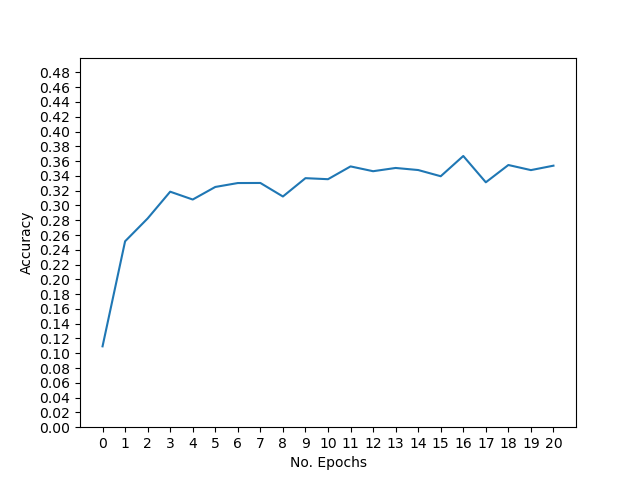
\includegraphics[width=0.5\textwidth]{"figures/fig_0.png"}} &
    \subfloat[mbs = 5,   lr = 0.1]{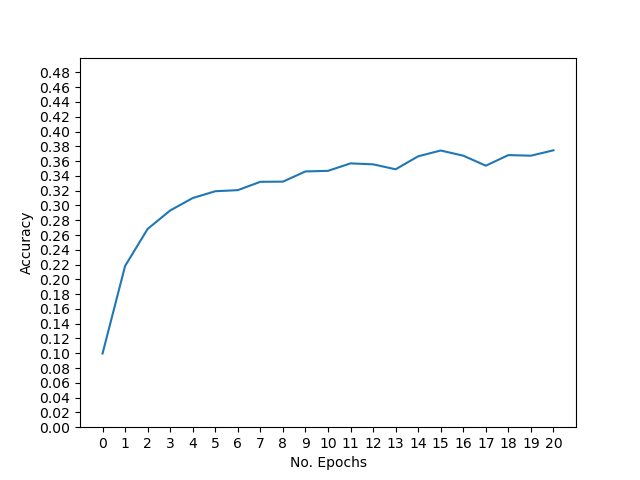
\includegraphics[width=0.5\textwidth]{"figures/fig_1.png"}} \\
    \subfloat[mbs = 20,  lr = 0.1]{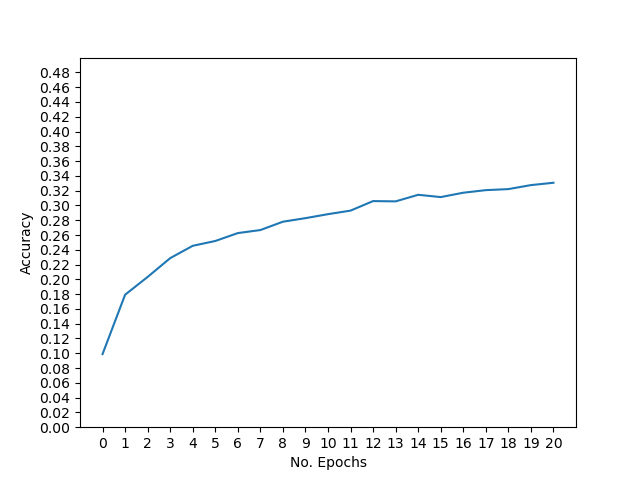
\includegraphics[width=0.5\textwidth]{"figures/fig_2.png"}} &
    \subfloat[mbs = 300, lr = 0.1]{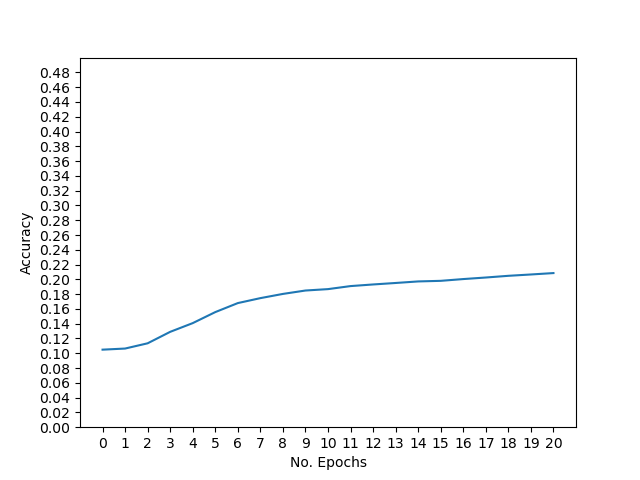
\includegraphics[width=0.5\textwidth]{"figures/fig_3.png"}} \\
    \end{tabular}
    \caption{Effect of mini-batch size on accuracy over epochs}
\end{figure}

\begin{figure}
    \centering
    \begin{tabular}{cc}
    \subfloat[mbs = 100, lr = 0.001]{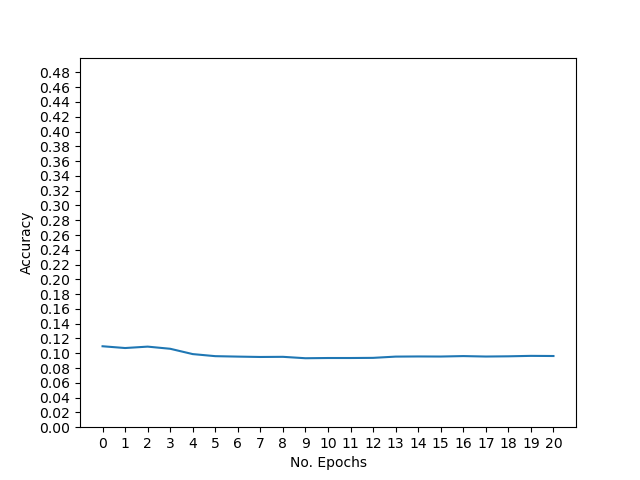
\includegraphics[width=0.5\textwidth]{"figures/fig_4.png"}} &
    \subfloat[mbs = 100, lr = 0.01 ]{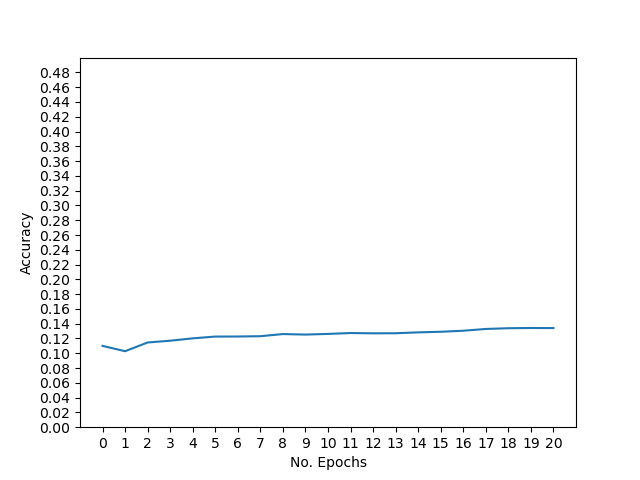
\includegraphics[width=0.5\textwidth]{"figures/fig_5.png"}} \\
    \subfloat[mbs = 100, lr = 0.1  ]{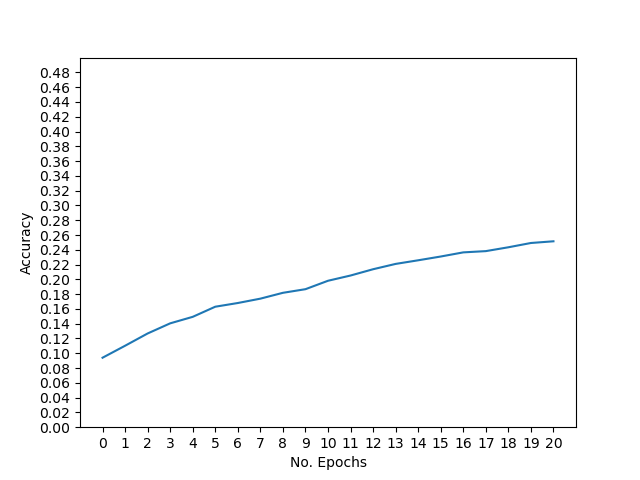
\includegraphics[width=0.5\textwidth]{"figures/fig_6.png"}} &
    \subfloat[mbs = 100, lr = 1.0  ]{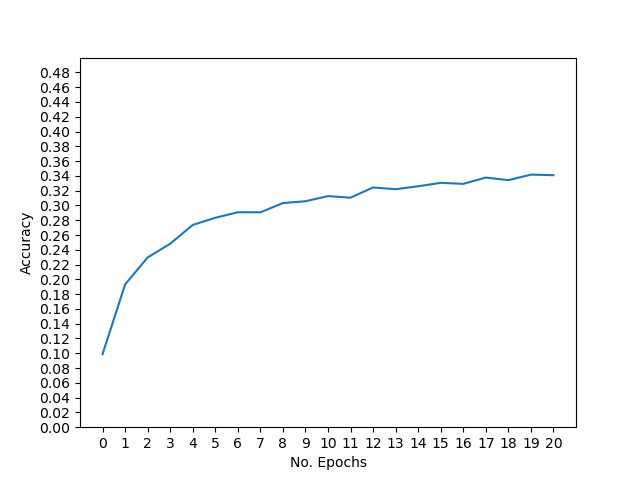
\includegraphics[width=0.5\textwidth]{"figures/fig_7.png"}} \\
    \subfloat[mbs = 100, lr = 10   ]{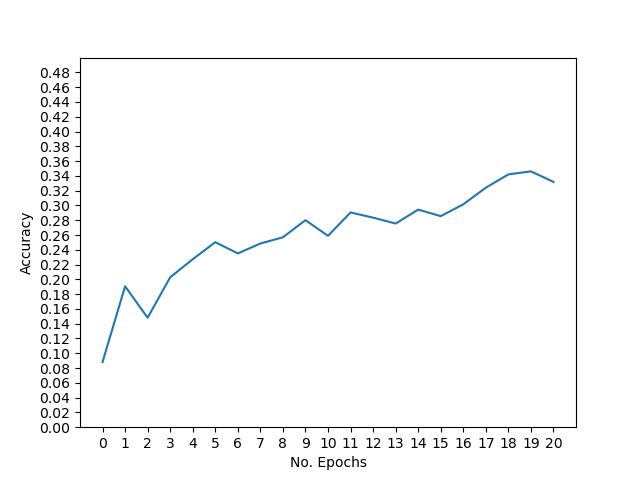
\includegraphics[width=0.5\textwidth]{"figures/fig_8.png"}} &
    \end{tabular}
    \caption{Effect of learning rate on accuracy over epochs}
\end{figure}


\newpage

\subsection{Findings}
Some text belongs here.


\section*{Conclusion}
Neural networks are good.

